\section{Domain Name System}
\subsection{Host names and IP Addresses}
\begin{itemize}[nosep]
    \item Host names
          \begin{itemize}[nosep]
              \item Mnemonics appreciated by humans
              \item Variable length, ASCII characters
              \item Provide little (if any) information about location
              \item Examples: www.facebook.com, bbc.co.uh
          \end{itemize}
    \item IP Addresses
          \begin{itemize}[nosep]
              \item Numerical address appreciated by routers
              \item Fixed length, binary numbers
              \item Hierarchical, related to host location (in the network)
              \item Examples: 69.171.228.14, 212.58.241.131
          \end{itemize}
\end{itemize}
\subsection{Separating Naming and Addressing}
\begin{itemize}[nosep]
    \item Names are easier to remember
          \begin{itemize}[nosep]
              \item www.cnn.com vs. 157.166.244.26
          \end{itemize}
    \item Addresses can change underneath
          \begin{itemize}[nosep]
              \item e.g. renumbering when changing providers
          \end{itemize}
    \item Name could map to multiple addresses
          \begin{itemize}[nosep]
              \item www.cnn.com maps to at least 6 IP addresses
              \item Enables
                    \begin{itemize}[nosep]
                        \item Load balancing
                        \item Latency reduction
                        \item Tailoring request based on requester's location/device/identity
                    \end{itemize}
              \item Multiple names for the same address
                    \begin{itemize}[nosep]
                        \item Aliases: www.cs.brown.edu and cs.brown.edu
                        \item Multiple servers in the same node (e.g. apache virtual servers)
                    \end{itemize}
          \end{itemize}
\end{itemize}
\subsection{Scalable Address \texorpdfstring{$\leftrightarrow$}{<->} Name Mappings}
\begin{itemize}[nosep]
    \item Original kept in a local file, \texttt{hosts.txt}
          \begin{itemize}[nosep]
              \item Flat namespace
              \item Central administrator kept master copy (for the internet)
              \item To add a host, emailed admin
              \item Downloaded file regularly
          \end{itemize}
    \item Completely impractical today
          \begin{itemize}[nosep]
              \item File would be huge (gigabytes)
              \item Traffic implosion (lookups and updates)
                    \begin{itemize}[nosep]
                        \item Some names change mappings every few days (dynamic IP)
                    \end{itemize}
              \item Single point of failure
              \item Impractical politics (repeated names, ownership, etc.)
          \end{itemize}
\end{itemize}
\subsection{Goals for an Internet-scale name system}
\begin{itemize}[nosep]
    \item Scalability
          \begin{itemize}[nosep]
              \item Must handle a huge number of records
                    \begin{itemize}[nosep]
                        \item With some software synthesizing names on the fly
                    \end{itemize}
              \item Must sustain update and lookup load
          \end{itemize}
    \item Distributed Control
          \begin{itemize}[nosep]
              \item Let people control their own names
          \end{itemize}
    \item Fault tolerance
          \begin{itemize}[nosep]
              \item Minimize lookup failures in face of other network problems
          \end{itemize}
\end{itemize}
\subsection{The Good News}
\begin{itemize}[nosep]
    \item Properties that make these goals easier to achieve
          \begin{enumerate}[nosep]
              \item Read-mostly database
                    \begin{itemize}[nosep]
                        \item Lookups \emph{much} more frequent than updates
                    \end{itemize}
              \item Loose consistency
                    \begin{itemize}[nosep]
                        \item When adding a machine, not end of the world if it takes minutes or hours to propagate
                    \end{itemize}
              \item These suggest aggressive caching
                    \begin{itemize}[nosep]
                        \item Once you've looked up a hostname, remember
                        \item Don't have to look again in the near future
                    \end{itemize}
          \end{enumerate}
\end{itemize}
\subsection{Domain Name System (DNS)}
\begin{figure}[H]
    \tikzsetnextfilename{dns-hierarchy}
    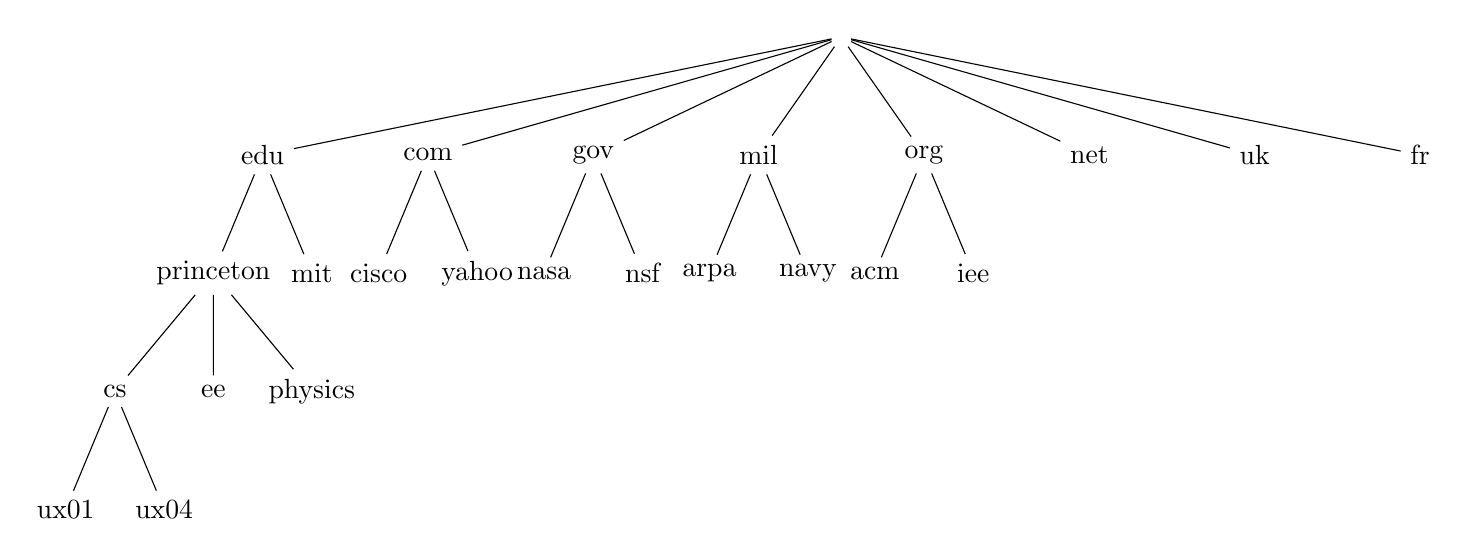
\begin{tikzpicture}[level 1/.style={sibling distance=2.1cm},level 2/.style={sibling distance=1.25cm}]
        \node{}
        child {node {edu}
                child {node {princeton}
                        child {node {cs}
                                child {node {ux01}}
                                child {node {ux04}}}
                        child {node {ee}}
                        child {node {physics}}}
                child {node {mit}} }
        child {node {com}
                child {node {cisco}}
                child {node {yahoo}}}
        child {node {gov}
                child {node {nasa}}
                child {node {nsf}}}
        child {node {mil}
                child {node {arpa}}
                child {node {navy}}}
        child {node {org}
                child {node {acm}}
                child {node {iee}}}
        child {node {net}}
        child {node {uk}}
        child {node {fr}};
    \end{tikzpicture}
\end{figure}
\begin{itemize}[nosep]
    \item Hierarchical namespace broken into \emph{zones}
          \begin{itemize}[nosep]
              \item root (.), edu., princeton.edu, cs.princeton.edu,
              \item Zones separately administred :: delegation
              \item Parent zone tells you how to find servers for subdomains
          \end{itemize}
    \item Each zone served from multiple replicated servers
\end{itemize}
\subsection{DNS Architecture}
\begin{itemize}[nosep]
    \item Hierarchy of DNS Servers
          \begin{itemize}[nosep]
              \item Root servers
              \item Top-level domain (TLD) servers
              \item Authoritative DNS servers
          \end{itemize}
    \item Performing the translation
          \begin{itemize}[nosep]
              \item Local DNS servers
              \item Resolver software
          \end{itemize}
\end{itemize}
\subsection{Resolver Operation}
\begin{itemize}[nosep]
    \item Apps make recursive queries to local DNS server
          \begin{itemize}[nosep]
              \item Ask server to get answer for you
          \end{itemize}
    \item Server makes iterative queries to remote servers
          \begin{itemize}[nosep]
              \item Ask servers who to ask next
              \item Cache results aggresively
          \end{itemize}
\end{itemize}
\begin{figure}[H]
    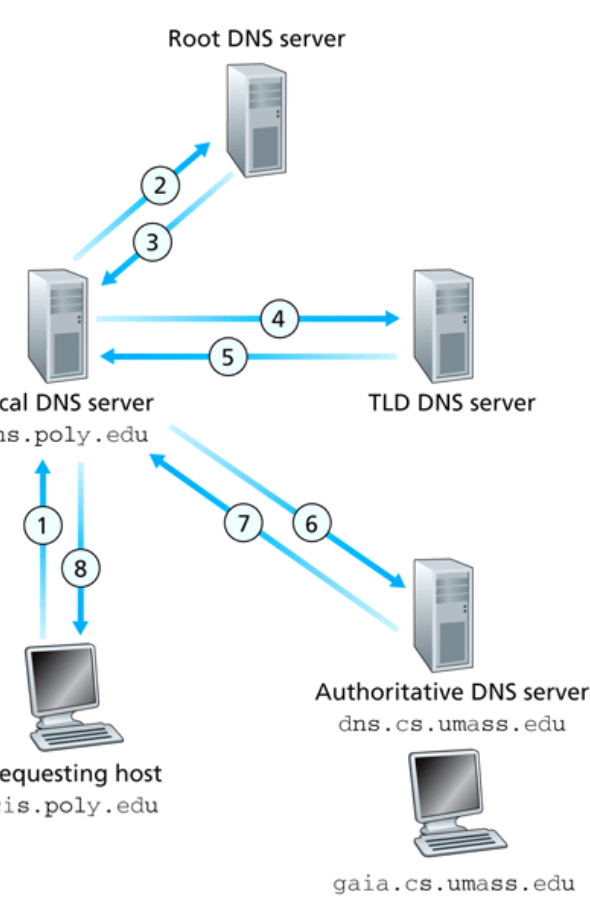
\includegraphics[width=0.25\textwidth]{lazy/resolveroperation.png}
\end{figure}
\subsection{DNS Root Server}
\begin{itemize}[nosep]
    \item Located in Virginia, USA
    \item How do we make the root scale?
\end{itemize}
\begin{figure}[H]
    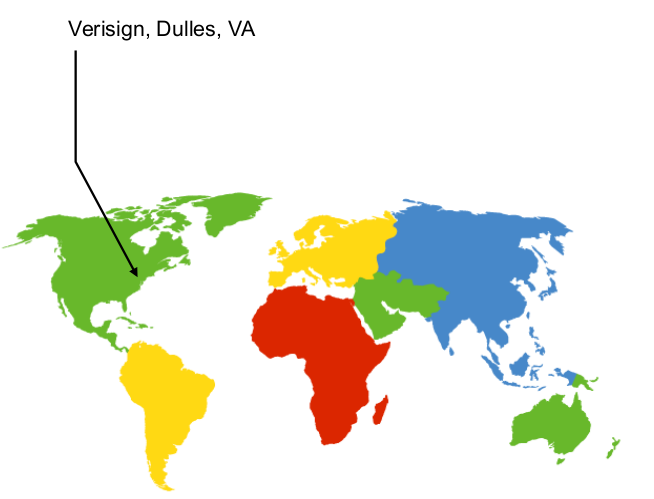
\includegraphics[scale=0.25]{lazy/dnsrootserver.png}
\end{figure}
\subsection{DNS Root Servers}
\begin{itemize}[nosep]
    \item 13 root servers (\url{www.root-servers.org})
          \begin{itemize}[nosep]
              \item Labeled A through M (e.g. A.ROOT-SERVERS.NET)
          \end{itemize}
    \item Does this scale?
          \begin{figure}[H]
              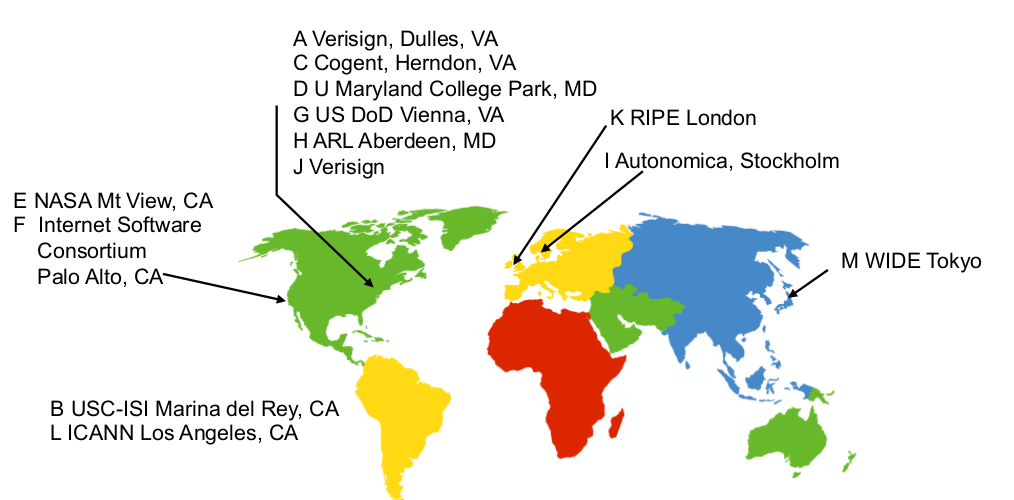
\includegraphics[scale=0.25]{lazy/dnsrootserver2.png}
          \end{figure}
    \item Replication via \emph{anycasting}
          \begin{figure}[H]
              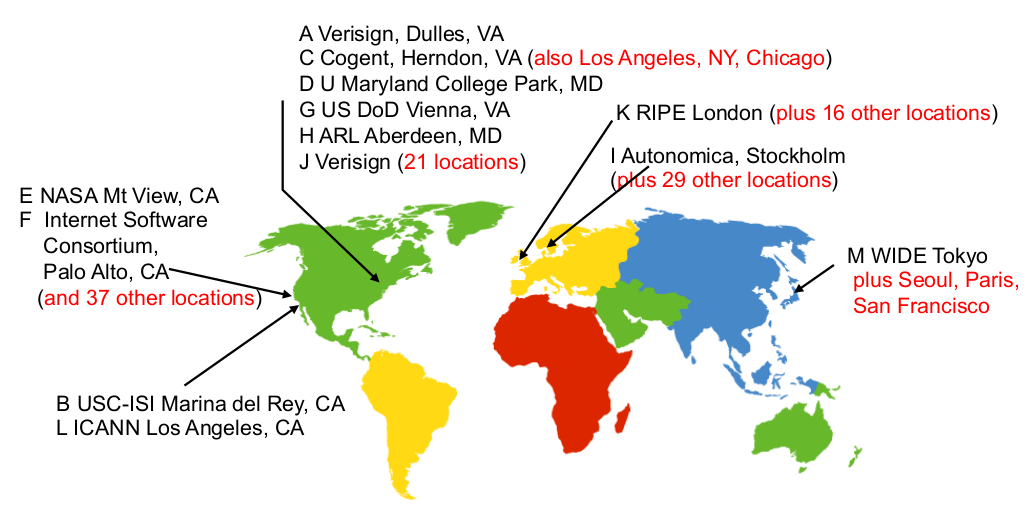
\includegraphics[scale=0.25]{lazy/dnsrootserver3.png}
          \end{figure}
\end{itemize}
\subsection{TLD and Authoritative DNS Servers}
\begin{itemize}[nosep]
    \item Top Level Domain (TLD) servers
          \begin{itemize}[nosep]
              \item Generic domains (e.g. com, org, edu)
              \item Country domains (e.g. uk, br, tv, in, ly)
              \item Special domains (e.g. arpa)
              \item Typically managed professionally
          \end{itemize}
    \item Authoritative DNS servers
          \begin{itemize}[nosep]
              \item Provides public records for hosts at an organization
                    \begin{itemize}[nosep]
                        \item e.g. for the organization's own servers (www, mail, etc)
                    \end{itemize}
              \item Can be maintained locally or by a service provider
          \end{itemize}
\end{itemize}
\subsection{Reverse Mapping}
\begin{itemize}[nosep]
    \item How do we get the other direction, IP address to name?
    \item Addresses have a hierarchy:
          \begin{itemize}[nosep]
              \item 128.148.34.7
          \end{itemize}
    \item But, most significant element comes first
    \item Idea: reverse the numbers, 7.34.148.128\dots
          \begin{itemize}[nosep]
              \item And look that up in DNS
          \end{itemize}
    \item Under what TLD?
          \begin{itemize}[nosep]
              \item Convention: in-addr.arpa
              \item Lookup 7.34.148.128.in-addr.arpa
              \item in6.arpa for IPv6
          \end{itemize}
\end{itemize}
\url{https://en.wikipedia.org/wiki/Reverse_DNS_lookup}
\subsection{DNS Caching}
\begin{itemize}[nosep]
    \item All these queries take a long time!
          \begin{itemize}[nosep]
              \item And could impose tremendous load on root servers
              \item This latency happens before any real communication, such as downloading your web page
          \end{itemize}
    \item Caching greatly reduces overhead
          \begin{itemize}[nosep]
              \item Top level servers very rarely change
              \item Popular sites visited often
              \item Local DNS server caches information from many users
          \end{itemize}
    \item How long do you store a cached response?
          \begin{itemize}[nosep]
              \item Original server tells you: TTL entry
              \item Server delete entry after TTL expires
          \end{itemize}
\end{itemize}
\subsection{Negative Caching}
\begin{itemize}[nosep]
    \item Remember things that don't work:
          \begin{itemize}[nosep]
              \item Misspellings like www.cnn.comm, ww.cnn.com
          \end{itemize}
    \item These can take a long time to fail for the first time
          \begin{itemize}[nosep]
              \item Good to cache negative results so it will fail faster next time
          \end{itemize}
    \item But negative caching is optional and not widely implemented
\end{itemize}
\subsection{DNS Protocol}
\begin{itemize}[nosep]
    \item TCP/UDP port 53
    \item Most traffic uses UDP
          \begin{itemize}[nosep]
              \item Lightweight protocol has 512 byte message limit
              \item Retry using TCP if UDP fails (e.g. reply truncated)
          \end{itemize}
    \item TCP requires message boundaries
          \begin{itemize}[nosep]
              \item Prefix all messages with 16-bit length
          \end{itemize}
    \item Bit in query determines if query is recursive
\end{itemize}
\subsection{Resource Records}
\begin{itemize}[nosep]
    \item All DNS info represented as resource records (RR) \[\text{\textcolor{blue}{name [ttl] [class] type rdata}}\]
          \begin{itemize}[nosep]
              \item name: domain name
              \item TTL: time to live in seconds
              \item class: for extensibility, normally IN (1) ``Internet''
              \item type: type for the record
              \item rdata: resource data dependent on the type
          \end{itemize}
    \item Two import RR types
          \begin{itemize}[nosep]
              \item A -- Internet Address (IPv4)
              \item NS -- name server
          \end{itemize}
    \item Example RRs
          \begin{minted}{html}
        bayou.cs.uh.edu. 3600 IN A 129.7.240.18
        cs.uh.edu. 3600 IN NS ns2.uh.edu.
        cs.uh.edu. 3600 IN NS dns.cs.uh.edu.
    \end{minted}
\end{itemize}
\subsection{Some important details}
\begin{itemize}[nosep]
    \item How do local servers find root servers?
          \begin{itemize}[nosep]
              \item DNS lookup on a.root-servers.net?
              \item Servers configured with \emph{root cache} file
              \item ftp://ftp.rs.internic.net/domain/db.cache
              \item Contains root name servers and their addresses
          \end{itemize}
    \item How do you get addresses of other name servers?
          \begin{itemize}[nosep]
              \item To obtain the address of www.cs.brown.edu, ask a.edu-servers.net, says a.root.servers.net
              \item How do you find a.edu-servers.net?
              \item Glue records: A records in parent zone.
          \end{itemize}
\end{itemize}